% interactcadsample.tex
% v1.04 - May 2023

\documentclass[]{interact}

\usepackage{epstopdf}% To incorporate .eps illustrations using PDFLaTeX, etc.
\usepackage{subfigure}% Support for small, `sub' figures and tables
%\usepackage[nolists,tablesfirst]{endfloat}% To `separate' figures and tables from text if required

\usepackage{natbib}% Citation support using natbib.sty
\bibpunct[, ]{(}{)}{;}{a}{}{,}% Citation support using natbib.sty
\renewcommand\bibfont{\fontsize{10}{12}\selectfont}% Bibliography support using natbib.sty

\theoremstyle{plain}% Theorem-like structures provided by amsthm.sty
\newtheorem{theorem}{Theorem}[section]
\newtheorem{lemma}[theorem]{Lemma}
\newtheorem{corollary}[theorem]{Corollary}
\newtheorem{proposition}[theorem]{Proposition}

\theoremstyle{definition}
\newtheorem{definition}[theorem]{Definition}
\newtheorem{example}[theorem]{Example}

\theoremstyle{remark}
\newtheorem{remark}{Remark}
\newtheorem{notation}{Notation}


% tightlist command for lists without linebreak
\providecommand{\tightlist}{%
  \setlength{\itemsep}{0pt}\setlength{\parskip}{0pt}}



\usepackage{hyperref}
\usepackage[utf8]{inputenc}
\def\tightlist{}


\begin{document}


\articletype{}

\title{Getting a Step Ahead: Using the Regularized Horseshoe Prior to
Select Cross-Loadings in Bayesian CFA}


\author{\name{A. N. Author$^{a}$, John Smith$^{b}$, Dominik
Leutnant$^{c, \dagger, \ddagger}$}
\affil{$^{a}$Taylor \& Francis, 4 Park Square, Milton Park, Abingdon,
UK; $^{b}$Institut für Informatik, Albert-Ludwigs-Universität, Freiburg,
Germany; $^{c}$Muenster University of Applied Sciences - Institute for
Infrastructure, Water, Resources, Environment, Correnstr. 25, 48149
Münster, Germany}
}

\thanks{CONTACT A. N.
Author. Email: \href{mailto:latex.helpdesk@tandf.co.uk}{\nolinkurl{latex.helpdesk@tandf.co.uk}}}
\thanks{CONTACT A. N.
Author. Email: \href{mailto:latex.helpdesk@tandf.co.uk}{\nolinkurl{latex.helpdesk@tandf.co.uk}}, John
Smith. Email: \href{mailto:john.smith@uni-freiburg.de}{\nolinkurl{john.smith@uni-freiburg.de}}, Dominik
Leutnant. Email: \href{mailto:leutnant@fh-muenster.de}{\nolinkurl{leutnant@fh-muenster.de}}}

\maketitle

\begin{abstract}
This is the first study to compare the Regularized Horseshoe Prior
(RHSP) to the Small Variance Normal Prior (SVNP) in their performance in
regularizing cross-loadings in Bayesian CFA. The SVNP can be used to
shrink cross-loadings in CFA to(wards) zero to identify models. This
often results in biased model estimates, as not only small, irrelevant,
but also large cross-loadings are shrunken substantially. The RHSP was
expected to regularize cross-loadings more efficiently, avoiding the
bias of the SVNP, by allowing large cross-loadings to escape shrinkage
within a single estimation step. It was found that indeed the SVNP had
overall higher levels of bias than the RHSP with large cross-loadings.
Hereby, the RHSP was robust across sample sizes, and different
hyper-parameter settings, although under some convergence failed.
Regarding the Power and Type-I-Error rate in selecting cross-loadings as
non-zero, both priors performed poorly, which is partially explained by
the low sample sizes considered.
\end{abstract}

\begin{keywords}
Regularization, Bayesian Regularized SEM, Small Variance Normal Prior,
Regularized Horseshoe Prior.
\end{keywords}

\begin{verbatim}
## Loading required package: tinylabels
\end{verbatim}

\begin{verbatim}
## -- Attaching core tidyverse packages ------------------------ tidyverse 2.0.0 --
## v dplyr     1.1.4     v readr     2.1.5
## v forcats   1.0.0     v stringr   1.5.1
## v lubridate 1.9.3     v tibble    3.2.1
## v purrr     1.0.2     v tidyr     1.3.1
## -- Conflicts ------------------------------------------ tidyverse_conflicts() --
## x lubridate::dst()      masks LaplacesDemon::dst()
## x dplyr::filter()       masks stats::filter()
## x lubridate::interval() masks LaplacesDemon::interval()
## x dplyr::lag()          masks stats::lag()
## x purrr::partial()      masks LaplacesDemon::partial()
## i Use the conflicted package (<http://conflicted.r-lib.org/>) to force all conflicts to become errors
## 
## Attaching package: 'jtools'
## 
## 
## The following object is masked from 'package:papaja':
## 
##     theme_apa
## 
## 
## 
## Attaching package: 'kableExtra'
## 
## 
## The following object is masked from 'package:dplyr':
## 
##     group_rows
## 
## 
## Loading required package: cmdstanr
## 
## This is cmdstanr version 0.7.1
## 
## - CmdStanR documentation and vignettes: mc-stan.org/cmdstanr
## 
## - CmdStan path: /home/michi/.cmdstan/cmdstan-2.34.1
## 
## - CmdStan version: 2.34.1
## 
## Loading required package: rstan
## 
## Loading required package: StanHeaders
## 
## 
## rstan version 2.32.6 (Stan version 2.32.2)
## 
## 
## For execution on a local, multicore CPU with excess RAM we recommend calling
## options(mc.cores = parallel::detectCores()).
## To avoid recompilation of unchanged Stan programs, we recommend calling
## rstan_options(auto_write = TRUE)
## For within-chain threading using `reduce_sum()` or `map_rect()` Stan functions,
## change `threads_per_chain` option:
## rstan_options(threads_per_chain = 1)
## 
## 
## 
## Attaching package: 'rstan'
## 
## 
## The following object is masked from 'package:tidyr':
## 
##     extract
## 
## 
## Loading required package: mvtnorm
## 
## 
## Attaching package: 'mvtnorm'
## 
## 
## The following object is masked from 'package:jtools':
## 
##     standardize
## 
## 
## The following objects are masked from 'package:LaplacesDemon':
## 
##     dmvt, rmvt
## 
## 
## Loading required package: parallel
## 
## Loading required package: bayesplot
## 
## This is bayesplot version 1.11.1
## 
## - Online documentation and vignettes at mc-stan.org/bayesplot
## 
## - bayesplot theme set to bayesplot::theme_default()
## 
##    * Does _not_ affect other ggplot2 plots
## 
##    * See ?bayesplot_theme_set for details on theme setting
\end{verbatim}

\hypertarget{introduction}{%
\section{Introduction}\label{introduction}}

The art of statistical modeling revolves around coming up with an
appropriate simplification, a \emph{model}, of a true
\emph{data-generating process}. Hereby, a fundamental trade-off between
model simplicity and model complexity arises, that is mostly known as
\emph{bias-variance trade-off}. Simple models with few parameters have
high bias, meaning that they deviate substantially from the true
data-generating process, and low variance, such that they generalize
well to other datasets from the same population. Complex models with
large numbers of parameters tend to have low bias and high variance.
They are thus prone to over-fitting, i.e., picking up patterns that are
only relevant in the dataset at hand, but do not generalize well to
other datasets. Moreover, complex models can be cumbersome to interpret
and often a large number of observations is required to estimate them
\citep{cox_principles_2006, james_introduction_2021}.

In confirmatory factor analysis \citep[CFA,][]{bollen_structural_1989}
it is common practice to deal with the bias-variance trade-off in a
brute-force manner, by imposing a so-called simple structure. Here,
cross-loadings, factor-loadings that relate items to factors that they
theoretically do not belong to, are fixed to zero to yield an identified
and easy to interpret model. This often leads to poor model fit, which
forces researchers to free some cross-loadings after the fact based on
empirical grounds (modification indices) to improve fit. This procedure
is flawed, as it risks capitalization on chance and thereby over-fitting
\citep{maccallum_model_1992}.

As a Bayesian solution to this issue \citet{muthen_bayesian_2012}
proposed identifying CFA models by setting the so-called \emph{Small
Variance Normal Prior} (SVNP) for cross-loadings, which is a normal
distribution with mean zero and a very small variance (e.g.,
\(\sigma^2\) = 0.01). This prior attaches large prior mass to
cross-loadings of or near zero, while attaching almost no prior mass to
cross-loadings further from zero, such that all cross-loadings in the
model are shrunken. However, shrinking also the cross-loadings that are
further from zero introduces substantial bias to the model
\citep{lu_bayesian_2016}. Consequently, Bayesian CFA requires a two-step
approach. First, the model is estimated with the SVNP set for the
cross-loadings and cross-loadings are selected as non-zero when their
95\% credible intervals do not contain zero
\citep{muthen_bayesian_2012}. The model is then re-estimated, where
cross-loadings that have been selected to be non-zero are freely
estimated without shrinkage, and the remaining cross-loadings are fixed
to zero, avoiding the bias in the model of the previous step. Correctly
selecting cross-loadings as non-zero can pose a challenge in practice,
as the performance of different selection criteria depends on a broad
set of conditions, making it difficult to formulate general
recommendations for researchers \citep{zhang_criteria_2021}. This calls
for shrinkage priors that allow us to `get a step ahead', by
regularizing cross-loadings in CFA models without causing substantial
bias, within a single estimation step.

One promising regularization prior that can be expected to allow
estimating CFA models with less bias within a single step is the
so-called Regularized Horseshoe Prior (RHSP), which is designed to let
large parameters escape shrinkage. While the Regularized Horseshoe Prior
has been shown to perform excellently in the selection of relevant
predictors in regression
\citep{piironen_sparsity_2017, van_erp_shrinkage_2019}, no previous
research has validated its performance in regularizing cross-loadings in
CFA. We therefore aim to compare the RHSP to the SVNP in their
performance in regularizing cross-loadings in Bayesian Regularized SEM.

In the remainder of this article we will first introduce regularization,
whereby we will discuss the advantages of Bayesian over frequentist
regularization. We will then outline Bayesian applications of
regularized SEM. Here we will explain different shrinkage priors in
detail, in particular the SVNP and the RHSP. Next, a simulation study is
reported that assesses the performance of the RHSP vs.~the SVNP in
selecting cross-loadings in a simple CFA model. We conclude by proposing
directions for future research in further establishing the usefulness of
the RHSP in Bayesian regularized SEM.

\hypertarget{theoretical-background}{%
\section{Theoretical Background}\label{theoretical-background}}

\hypertarget{regularization}{%
\subsection{Regularization}\label{regularization}}

A classic method of trying to find a balance between model complexity
and model simplicity is \emph{regularization}
\citep{hastie_statistical_2015}. Regularization entails adding some bias
to a model on purpose to reduce its variance. This helps to make models
easier to interpret and more generalizable. In a frequentist context,
regularization is achieved by adding a so-called penalty term to the
cost function of a model. This ensures that model parameters that are
irrelevant, e.g., small regression coefficients in a regression model
with a large number of predictors, are shrunken to (or towards) zero.
For a regression model, where we predict N individual scores i on an
outcome \(y_i\) based on scores on a vector of predictors \(x_i\), the
vector of regression coefficients \(\beta\), and a random error term
\(e_i\): \[y_i = \beta x_i + e_i, \ \text{where} \]
\[e_i \sim \mathcal{N}(0, \sigma^2). \] The Ordinary Least Squared
Residuals estimates of \(\beta\) are obtained by minimizing the sum of
squared residuals:
\[ \hat{\beta} = \underset{\beta}{argmin} \{ \Sigma_{i=1}^N(y_i - \beta x_{i} )^2 \}.\]
Penalized regression adds a a penalty term to this cost function, which
is generally denoted as \(||\beta||_L\):
\[ \hat{\beta} = \underset{\beta}{argmin} \{ \Sigma_{i=1}^N(y_i - \beta x_{i} )^2 + \lambda ||\beta||_{L} \}.\]
When L = 1, we speak of the so-called L-1 norm. In this case the penalty
is: \(||\beta||_1 = \Sigma_{j=1}^p |\beta_j|\). This is the well-known
LASSO (Least Absolute Shrinkage and Selection Operator) penalty
\citep{tibshirani_regression_1996, tibshirani_regression_2011}. Here,
the absolute values of the regression coefficients are added up,
multiplied by \(\lambda\), and then added to the sum of the squared
errors within the model's cost-function. The basic intuition is as
follows. Just as minimizing the sum of the (squared) residuals leads to
estimates of the model parameters with minimally small residuals,
minimizing the (absolute) sum of the regression coefficients results in
smaller values of the regression coefficients. The larger \(\lambda\),
the more weight the penalty has, and thereby the higher the amount of
shrinkage to(wards) zero. In practice the hyper-parameter \(\lambda\) is
often determined by means of cross-validation. When L = 2 (the so-called
L2-norm), \(||\beta||_2 = \sqrt{\Sigma_{j=1}^p \beta_j^2}\). This is the
famous ridge penalty \citep{hoerl_ridge_2000}. Here, the same general
principle is followed. This time not the absolute sum, but the square
root of the sum of squares of the regression coefficients is minimized.
In practice, one key difference between the LASSO and the ridge penalty
is that the former shrinks some coefficient entirely to zero (thereby
actively selecting predictors), whereas in ridge regression coefficients
are only shrunken approximately but never entirely to zero.

Regularization can also be applied in more complex models, which is
illustrated by the body of literature applying regularization in
Structural Equation Modeling (SEM). Regularized SEM entails adding
penalties to the cost function of SEM models (typically a variant of the
maximum likelihood cost function, \(F_{ML}\)) to reach sparser models.
Now, for any given set of model parameters \(\theta\), we can add a
penalty function \(P(\theta)\) to the cost function of the model:
\[F_{ML, \ penalized} = F_{ML} \ + \lambda P(\theta).\] Again the
penalty function can take on different forms, such as the ridge (the
square root of the sum of squares of the parameters) or the LASSO (the
sum of the absolute values of the parameters), and \(\lambda\) is again
a hyper-parameter that determines the amount of shrinkage. Regularized
SEM has successfully been applied in selecting cross-loadings and
residual covariances in CFA, especially under favorable conditions such
as large sample sizes \citep{jacobucci_regularized_2016}. Also
structural model parameters, such as regression coefficients in MIMIC
models \citep{jacobucci_regularized_2016, jacobucci_practical_2019}, or
indirect effects in mediation models with continuous
\citep{serang_exploratory_2017} or dichotomous outcomes
\citep{serang_exploratory_2020}, have successfully been regularized
through the usage of penalties such as the LASSO or ridge penalty.

The key disadvantage of the frequentist regularization approach is that
it depends on optimization. With more complicated penalties, and in
particular for complex models, it can be hard to derive optimizable cost
functions in practice. Also the derivation of unbiased standard errors
is often challenging under such circumstances, which hinders reliable
inference \citep{jacobucci_regularized_2016, jacobucci_comparison_2018}.
Bayesian approaches to regularization overcome these obstacles
\citep{jacobucci_comparison_2018}. In Bayesian model estimation, the
so-called Joint Posterior Distribution of the model parameters given the
data is a combination of the data given the model parameters (the
likelihood) and the prior distribution of the model parameters, i.e.,
\[P({\theta} | data) \sim  P(data | \theta) P(\theta) .\] Priors can
therefore be used to shrink model parameter estimates to(wards) zero.
Such priors are called a shrinkage prior. In the most simple case one
can simply set a normal prior for parameters that is centered around
zero (as the SVNP mentioned above), which resembles the ridge penalty
\citep{hsiang_bayesian_1975}. The LASSO penalty can be mimicked by
setting a Laplace- (double exponential) prior for parameters
\citetext{\citealp{park_bayesian_2008}; \citealp{hans_bayesian_2009}; \citealp[see][
for the Bayesian equivalents of other relevant
penalties]{van_erp_shrinkage_2019}}. The fact that in Bayesian inference
the whole joint posterior distribution of the model parameters can be
sampled by means of Markov chain Monte Carlo (MCMC) methods poses a
central advantage. This renders it unnecessary to derive standard
errors, as the variance of the posterior distribution of model
parameters is directly available. Also complex shrinkage priors with
unique desired properties can be implemented without having to yield an
optimizable cost-function, making Bayesian regularization a very
flexible approach.

\hypertarget{bayesian-cfa-and-the-small-variance-normal-prior-svnp}{%
\subsection{Bayesian CFA and The Small Variance Normal Prior
(SVNP)}\label{bayesian-cfa-and-the-small-variance-normal-prior-svnp}}

Confirmatory Factor Analysis \citep[CFA,][]{bollen_structural_1989} is
an essential tool for modeling measurement structures, falling under the
class of Structural Equation Models (SEM). For every individual i, the
scores on a vector of \(p \times 1\) observed indicators \(y_i\) is
modeled as follows:
\[\boldsymbol{y}_i = \boldsymbol{\mu} + \Lambda \boldsymbol{\eta}_i + \boldsymbol{e}_i ,\]
where \(\boldsymbol{\mu}\) is a \(p \times 1\) vector of intercepts,
\(\Lambda\) is a \(p \times q\) matrix of factor-loadings,
\(\boldsymbol{\eta}_i\) is a \(q \times 1\) vector of scores on the q
latent factors, and \(\boldsymbol{e}_i\) is a \(p \times 1\) vector of
random (measurement) error terms. Here, \(\Lambda\) is thus the part of
the equation that relates the latent variables to the observed scores on
the items.

We can differentiate between so-called main-loadings, and
cross-loadings. The former are factor-loadings that relate factors and
items to one another that are theoretically expected to have a
relationship. Cross-loadings are factor-loadings that relate factors to
items between which, theoretically, no relationship should exist. One
key property of CFA is that a clear expectation on the factor structure,
i.e., which factor loads on which items, is assumed. This allows to
formulate clear expectations on which items can be viewed as
cross-loadings. Consequently, a natural way of identifying CFA (on top
of other relevant identification constraints, such as scaling the
factors) is to fix all cross-loadings to zero. Not only does that
identify models, but it also ensures that the measurement structure is
easy to interpret. However, in practice, fixing all cross-loadings to
zero often results in poor model fit. So-called modification indices can
be derived, which indicate how much model-fit improves when adding or
removing a certain parameter (for instance, a cross-loading) to the
model. Based on modification indices, researchers often re-add some
cross-loadings to the model, until a desired level of fit is reached.
However, a core property of modification indices is that they are only
based on the dataset at hand, and may therefore only pick up noise that
is not relevant in the underlying population. Identifying cross-loadings
based on modification indices thus risks capitalization on chance.
Consequently, measurement structures may be selected that do not
generalize well to other datasets from the same population, hence
over-fitting may occur \citep{maccallum_model_1992}.

As solution to this issue, \citet{muthen_bayesian_2012}, proposed a
Bayesian way of identifying CFA models. They argued that fixing
cross-loadings of factor j on item k \(\lambda_{c,jk}\) to zero can be
interpreted as setting a normal prior with both a mean and a variance of
zero on them: \[\lambda_{c,jk}  \sim \mathcal{N}(0, \ 0).\] Now, since
usually most cross-loadings are indeed zero, but there are some that are
a bit larger (in absolute terms) than zero, and few that are
substantially larger, a more realistic prior would be a normal
distribution that is still centered around zero, but does have a small
variance, e.g.,\\
\[\lambda_{c,jk}  \sim \mathcal{N}(0, \ 0.01).\] The intuition of
setting such a prior, which we refer to as Small Variance Normal Prior
(SVNP), becomes clear when looking at Figure 1. In Bayesian model
estimation the prior of a parameter directly influences the final
posterior parameter estimate. By assuming that most cross-loadings are
zero, most posteriors of cross-loadings will be centered around zero. At
the same time, the prior allows for some deviations from zero, as there
is also some prior mass for cross-loadings that are marginally larger or
smaller than zero. Of course, applying the SVNP as prior for
cross-loadings is thus nothing but a Bayesian variant of Regularized
SEM, which strongly resembles the frequentist ridge penalty that was for
instance applied by \citet{jacobucci_regularized_2016}.

In practice an issue arises with the Bayesian CFA method, once
substantially large cross-loadings enter the picture. The estimates of
truly large cross-loadings should be large, as otherwise the
(co-)variance structure of the data is not explained properly. With the
SVNP, however, the estimates of large cross-loadings are also shrunken
substantially to(wards) zero, as the prior with its thin tails attaches
no prior mass to them. This causes bias. First, bias naturally occurs in
the large cross-loadings itself. However, also in other parameters, such
as factor-correlations or main-loadings, substantial bias can arise, as
they are estimated conditionally on the cross-loadings. To overcome
this, the method is presented as a 2 step-approach
\citep{muthen_bayesian_2012}. First, the model is estimated with the
shrinkage prior set for the cross-loadings. Cross-loadings are then
selected as non-zero if their 95\% credible interval does non contain
zero. Then the model is re-estimated. The as non-zero selected
cross-loadings are estimated freely without shrinkage, avoiding the bias
in their estimates of the previous step. The as zero selected
cross-loadings are fixed to zero.

\hypertarget{alternative-shrinkage-priors}{%
\subsection{Alternative Shrinkage
Priors}\label{alternative-shrinkage-priors}}

One alternative to the SVNP is the Bayesian LASSO, which has
successfully been applied in regularized SEM previously
\citep{chen_jinsong_partially_2021, zhang_criteria_2021}. In general,
its performance is similar to that of the SVNP. While a core difference
between the ridge- and the LASSO penalty is that the LASSO penalty
automatically shrinks some parameters to zero, the Bayesian equivalent
of the LASSO also requires manual selection. This is because Bayesian
model estimates, posterior means, will never be entirely zero
\citep{zhang_criteria_2021}. As the SVNP, the Laplace prior of the
Bayesian LASSO has thin tails, though slightly thicker than those of the
SVNP, attaching only little prior mass to large cross-loadings.
Consequently, as with the SVNP, a two-step approach is required to
estimate parameters without bias. \citet{zhang_criteria_2021} pointed
out that it is difficult to formulate general recommendations on how to
best select cross-loadings as non-zero when applying the Bayesian LASSO.
It is thus desirable to find regularization priors that can be applied
in Bayesian CFA that allow for estimating model parameters without bias
within a single step, to overcome the dependence on correctly selecting
cross-loadings.

One suitable alternative regularization prior for the purpose of
selecting cross-loadings in regularized Bayesian SEM is the so-called
Spike-and-Slab Prior
\citep{george_variable_1993, ishwaran_spike_2005, mitchell_bayesian_1988}.
This prior is a discrete mixture of an extremely peaked prior around
zero (the spike), and a very flat prior for larger parameters (the
slab). Formally, and applied to the cross-loadings in CFA, for every
cross-loading of factor j on item k, the Spike-and-Slab Prior can be
specified as (Lu et al., 2016):
\[\lambda_{c,jk} |r_{jk} \sim (1 \ - \ r_{jk})\delta_0 + r_{jk} \mathcal{N}(0, c^2_{jk}) , \ \text{with}\]
\[r_{jk} \sim \mathcal{Bernoulli}(p_{jk}).\] The basic intuition is as
follows. When \(r_{jk} = 1\),
\(\lambda_{c,jk} \sim \mathcal{N}(0, c^2_{jk})\), hence
\(\lambda_{c,jk}\) is assigned to the slab. When \(r_{jk} = 0\),
\(\lambda_{c,jk} \sim \delta_0\). In this case, the cross-loading is
thus assigned to a point-mass at zero, i.e., it is assigned to the
spike. This ensures that large cross-loadings that are relevant are not
shrunken while small, negligible cross-loadings are shrunken to zero. Lu
et al.~(2016) found that Spike-and-Slab Prior performs well in shrinking
truly zero cross-loadings to zero, while not shrinking (relevant) large
cross-loadings to avoid bias, especially under favorable conditions with
large sample sizes and cross-loadings. The prior is thus in general more
suited to estimate CFA models without substantial bias within a single
estimation step, due to its refined nature in differentiating between
large and small cross-loadings. However, the Spike-and-Slab Prior cannot
be implemented in STAN, one of the most popular software package for
MCMC-sampling, as STAN does not allow for discrete mixture priors
\citep{stan_development_team_stan_2021, betancourt_conceptual_2018}.
This calls for a \emph{non-discrete} alternative shrinkage prior that
also outperforms the SVNP within a single estimation step.

\hypertarget{the-regularized-horseshoe-prior-rhsp}{%
\subsection{The Regularized Horseshoe Prior
(RHSP)}\label{the-regularized-horseshoe-prior-rhsp}}

A fully continuous alternative to the Spike-and-Slab Prior that is
implementable in STAN is the so-called \emph{Regularized Horseshoe
Prior}
\citep[RHSP,][]{piironen_hyperprior_2017, piironen_sparsity_2017}. This
prior is an extension of the Horseshoe Prior
\citep{carvalho_horseshoe_2010}. The main idea of the original Horseshoe
Prior is that there is a \emph{global shrinkage parameter} \(\tau\),
shrinking all cross-loadings to zero. Next to this, there is a
\emph{local shrinkage parameter} \(\bar{\omega}_{jk}\)\footnote{We
  deviate from the common notation of the local shrinkage parameter as
  \(\bar{\lambda}\), as this letter is commonly used to denote
  factor-loadings in CFA.} that allows truly large cross-loadings to
escape the shrinkage, by setting thick Cauchy tails for the local scales
\(\omega_{jk}\) \citep{polson_shrink_2010}. Formally, the Horseshoe
prior for every cross-loading of factor j on item k is specified as
follows:
\[\lambda_{c,jk} | \omega_{jk}, \tau, c\sim \mathcal{N}(0, \ \omega^2_{jk} \tau^2), \ \text{where}\]
\[\omega_{jk} \sim \mathcal{C^+}(0, 1).\] The name-giving intuition
behind the horseshoe prior becomes clear when considering the finding
that a so-called shrinkage factor \(k_{jk}\) can be derived for the
individual cross-loadings
\citep{carvalho_horseshoe_2010, piironen_sparsity_2017}. This shrinkage
factor ranges from zero to one, with zero meaning no, and one meaning a
lot of shrinkage. When plotting the density of \(k_{jk}\) there is a
very high peak at low values and a very high peak at high values,
resulting in a plot that resembles a horseshoe, illustrating that the
Horseshoe Prior has the desired property of either shrinking parameters
very little, or very much, with very few parameters that are shrunken in
a non-extreme fashion.

The Horseshoe Prior was found consistently to possess the theoretical
properties of not shrinking large parameters while shrinking small
parameters substantially to zero in practice
\citep{carvalho_horseshoe_2010, polson_shrink_2010, datta_asymptotic_2013, van_der_pas_horseshoe_2014}.
However, due to its heavy Cauchy tails it suffers from the same issues
as a Cauchy prior. Specifically, not shrinking large parameters at all
can lead to estimation issues, especially when parameters are weakly
identified. This happens for instance in logistic regression with
separable data, where a flat likelihood and thereby a weakly identified
model arises \citep{ghosh_use_2018}. The RHSP prevents such issues by
shrinking also large parameters a little bit. The RHSP is specified as
follows. For every cross-loading of factor j on item k:
\[\lambda_{c,jk} | \bar{\omega}_{jk}, \tau, c\sim \mathcal{N}(0, \ \bar{\omega}^2_{jk} \tau^2), \ \text{with} \ \bar{\omega}^2_{jk} = \frac{c^2\omega_{jk}^2}{c^2 + \tau^2 \omega_{jk}^2},\]
\[\tau | df_{global}, s_{global} \sim half-t_{df_{global}}(0,\  s_{global}^2), \ \text{with} \  s_{global} = \frac{p_0}{p-p_0}\frac{\sigma}{\sqrt{N}},\]
\[\omega_{jk}| df_{local}, s_{local} \sim half-t_{df_{local}}(0, \ s_{local}^2),\]
\[c^2 | df_{slab}, s_{slab} \sim \mathcal{IG}(\frac{df_{slab}}{2}, \  df_{slab} \times \frac{s_{slab}^2}{2}),\]
where \(p_0\) represents a prior guess of the number of relevant
cross-loadings. Allowing to incorporate prior expectations on the
expected number of non-zero parameters is another core advantage of the
RHSP over the original Horseshoe Prior. However, it is not necessary to
use \(p_0\). One can simply set \(s_{global}\) manually, whereby it is
worth to consider that a \(s_{global}\) created based on a \(p_0\) will
typically be much lower than 1 \citep{piironen_sparsity_2017}. Note that
we specify the RHSP in its most general form. Setting the degrees of
freedoms of the half-t-distributions to 1 results in half-Cauchy
distributions. Strictly speaking, the prior is only a Regularized
\emph{Horseshoe} Prior when this is the case. In the current study we
vary the degrees of freedoms of all scale parameters to assess the
extent to which the sparcifying properties as well as the convergence of
the RHSP are influenced by this.

The intuition of how the RHSP shrinks large parameters a little bit is
best illustrated by assuming that c is a given constant. Now, when
\(\tau^2 \omega^2_{jk} < c^2\),
\(\bar{\omega}^2_{jk} \to \omega^2_{jk}\). Hence, in this case the RHSP
approaches the original Horseshoe Prior, with equally pronounced
shrinkage to zero. However, when \(\tau\) is far from zero, hence under
large true cross-loadings, \(\tau^2 \omega^2_{jk} > c^2\), and
\(\bar{\omega}^2_{jk} \to \frac{c^2}{\tau^2}\). Then, the prior of
\(\lambda_{c,jk}\) approaches a slab \(\mathcal{N}(0, c^2)\). Under the
above specification, when c is no constant but a parameter for which an
Inverse-Gamma hyper-prior is set, the slab becomes a t-distribution with
\(df_{slab}\) degrees of freedom, a mean of zero and a scale of
\(s_{slab}^2\) \citep{piironen_sparsity_2017}.

\begin{figure}
\centering
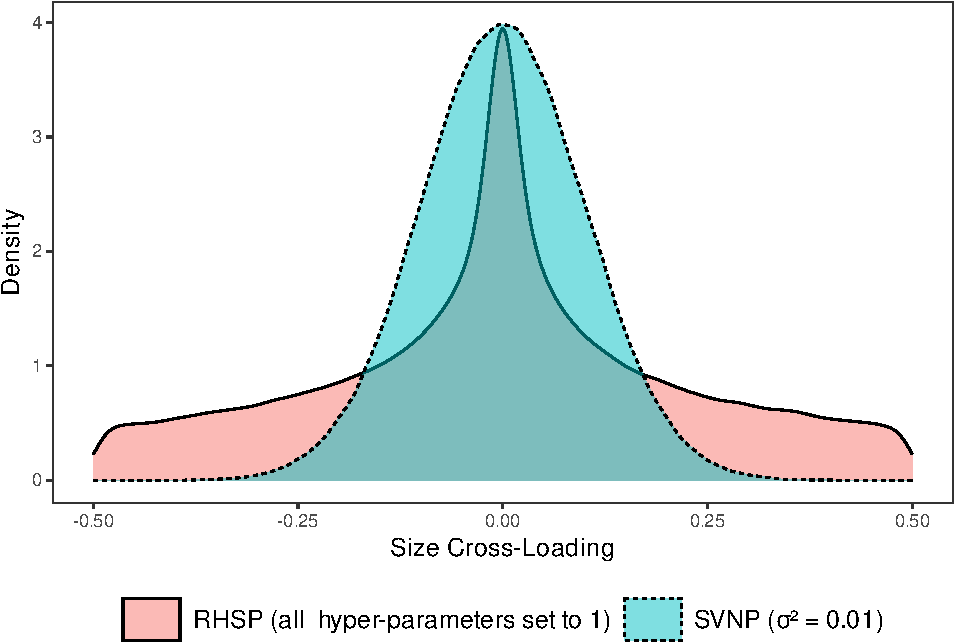
\includegraphics{Koch-vanErp_files/figure-latex/unnamed-chunk-1-1.pdf}
\caption{Density Plots of the Regularization Priors of Interest.}
\end{figure}

Figure 1 compares the two shrinkage priors that are the focus of our
study. Both priors share a large peak at zero, which ensures that
cross-loadings are shrunken to(wards) zero. However, the RHSP has much
thicker tails. Here, for larger cross-loadings, there is thus much more
prior mass than with the SVNP. This ensures large cross-loadings (and
consequently other model parameters) can be estimated without bias
within a single estimation step.

\hypertarget{the-current-study}{%
\section{The current study}\label{the-current-study}}

\hypertarget{study-procedure-and-parameters}{%
\subsection{Study Procedure and
Parameters}\label{study-procedure-and-parameters}}

A Monte Carlo simulation study was conducted using STAN
\citep{stan_development_team_stan_2021} and R
\citep{r_core_team_r_2021}. We used \texttt{cmdstandr} to interface STAN
with R \citep{gabry_cmdstanr_2022}, while also heavily relying on
\texttt{rstan} \citep{stan_development_team_rstan_2022} and
\texttt{bayesplot} \citep{gabry_bayesplot_2022} for the post-processing
of the posterior samples. Results were further post-processed using
\texttt{tidyr} \citep{wickham_tidyr_2022} \& \texttt{dplyr}
\citep{wickham_dplyr_2022}. All plots were made using \texttt{ggplot2}
\citep{wickham_ggplot2_2016}. We ran up to 46 replications in parallel
using the \texttt{parallel} package \citep{r_core_team_package_2022}.
This manuscript was written using R Markdown and the \texttt{papaja}
package \citep{aust_papaja_2022}. All code that was used to run the
simulations can be openly accessed on the author's
\href{https://github.com/JMBKoch/1vs2StepBayesianRegSEM}{\textbf{github}}\footnote{Specifically,
  the R-scripts needed to run the simulation can be found on
  \url{https://github.com/JMBKoch/1vs2StepBayesianRegSEM/tree/main/R}.
  \texttt{parameters.R} can be adjusted to adjust study parameters, and
  \texttt{main.R} is used to run the main simulation. Required packages
  are listed at the top of \texttt{parameters.R}.}. The models were
sampled using the No-U-Turn-Sampler \citep{homan_no-u-turn_2014}, with
two chains, a burnin-period of 2000 and a chain-length of 4000. These
sampling parameters were identified in pilot runs to be required for the
RHSP to reach convergence, and were therefore also used for the SVNP in
order to ensure a fair comparison.

\hypertarget{conditions}{%
\subsection{Conditions}\label{conditions}}

\hypertarget{population-conditions}{%
\subsubsection{Population Conditions}\label{population-conditions}}

The datasets were simulated based on a true 2-factor model, with three
items per factor, and a factor correlation of 0.5. The true model is
summarized below, both in equations (Appendix A) and graphically (Figure
2).\footnote{The STAN code of the model can be found on
  \url{https://github.com/JMBKoch/1vs2StepBayesianRegSEM/blob/main/stan/}.}
The factors were scaled by fixing their means to zero and their
variances to 1. All main-loadings were set to 0.75, and all residual
variances to 0.3, to ensure that the largest proportion of variance in
the items would be explained by their corresponding factor. We varied
the size of the two truly non-zero cross-loadings \(\lambda_{c 1}\) and
\(\lambda_{c 6}\) between 0.2, a negligible magnitude such that
shrinkage to zero is desired, and 0.5, a size for which shrinkage
towards zero should be avoided. We varied the sample sizes of the
simulated datasets between N = 100 and N = 200. Larger sample sizes of
for instance 500 were not included despite being common place in
previous simulation studies, because adding them would have rendered the
run-time of the simulations for the RHSP unfeasible. This is appropriate
because for simple factor models applied researchers are unlikely to
collect such larger sample sizes in practice, such that our findings
still generalize to real-life settings.

For all parameters except the cross-loadings, non-informative priors
were set: for the main-loadings a normal prior with mean of zero and a
variance of 25, for the residual variances a half-Cauchy-prior with a
location-parameter of 0 and a scale of 5, and for the factor-correlation
STAN's default uniform prior.

\hypertarget{svnp-prior-conditions}{%
\subsubsection{SVNP: Prior Conditions}\label{svnp-prior-conditions}}

We varied the hyper-parameter of the SVNP, \(\sigma^2\), between 0.001,
0.01 and 0.1, based on \citet{muthen_bayesian_2012}. For the SVNP this
left us with a total number of 2 (size cross-loading) x 2 (N) x 3
(hyper-parameter \(\sigma^2\)) = 12 individual conditions. Per
condition, 200 replications were run, yielding a total of 2400
replications for this prior.

\begin{figure}
\centering
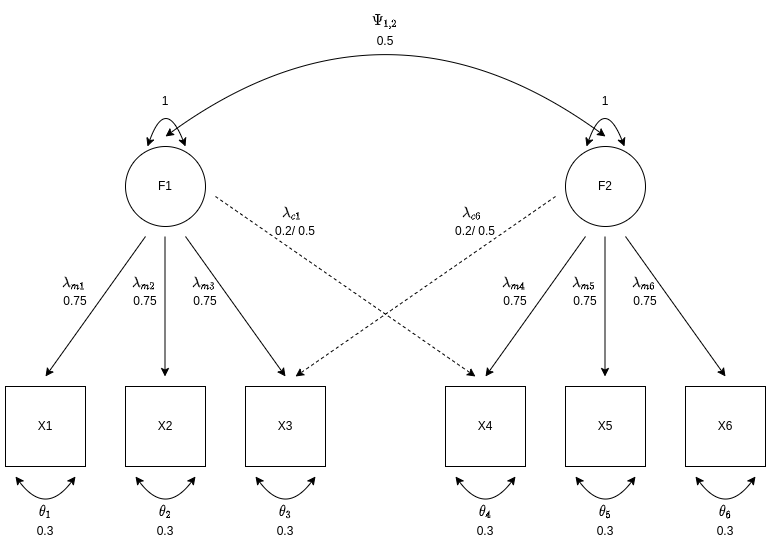
\includegraphics{~/1vs2StepBayesianRegSEM/Rmd/figures/model.png}
\caption{Graphical Representation of the True Model.}
\end{figure}

\hypertarget{rhsp-prior-conditions}{%
\subsubsection{RHSP: Prior Conditions}\label{rhsp-prior-conditions}}

The RHSP has six hyper-parameters in the specification that we apply. We
varied the scale of the global shrinkage parameter \(\tau\),
\(s_{global}\) between, 0.1 and 1. Here 1, is a natural maximum given
that the scale generally does not become larger than 1 when applying a
prior guess \(p_0\) \citep{piironen_sparsity_2017}, and 0.1 a logical
minimum given the (standardized) scale of the model. Also the scale of
the local shrinkage parameter \(\omega_{jk}\) was varied between, 0.1
and 1. The degrees of freedoms of these two parameters, \(df_{local}\)
and \(df_{global}\) were varied between 1 and 3. Larger degrees of
freedoms may help to overcome sampling issues that can arise when the
df's are set to one. Finally, for the scale of the distribution of
\(c^2\), \(s_{slab}\) was varied between 0.1, 1 and 5, and \(df_{slab}\)
between 1 and 3. We decided to include a broader range of scales for the
slab, as the slab is crucial in determining the shrinkage of large
cross-loadings. We were thus left with
\(2 \ (s_{global}) \times 2 \ (df_{global}) \times \ 2 \ (s_{local}) \times2 \ (df_{local}) \times 3 \ (s_{slab}) \times2 \ (df_{slab}) = 96\)
hyper-parameter conditions for the RHSP. In combination with the
\(2 \times 2\) population conditions this yielded 384 individual
conditions for this prior. In total there were thus
\(384 \times 200 = 76800\) replications run for the RHSP. Table 1
summarizes all conditions.

\begin{verbatim}
## Loading required package: tinylabels
\end{verbatim}

\begin{table}[tbp]

\begin{center}
\begin{threeparttable}

\caption{\label{tab:unnamed-chunk-2}Overview study conditions.}

\begin{tabular}{lll}
\toprule
Condition & \multicolumn{1}{c}{Levels} & \multicolumn{1}{c}{Values}\\
\midrule
$\bf{Population}$ &  & \\
Sample size (N) & 2 & 100, 200\\
Size cross-loading $\lambda_{c1 , 6}$ & 2 & 0.2, 0.5\\
\bf{SVNP} &  & \\
$\sigma^2$ & 3 & 0.1, 0.01, 0.001\\
\bf{RHSP} &  & \\
$s_{global}$ & 2 & 0.1, 1\\
$df_{global}$ & 2 & 1, 3\\
$s_{local}$ & 2 & 0.1, 1\\
$df_{local}$ & 2 & 1, 3\\
$s_{slab}$ & 3 & 0.1, 1, 5\\
$df_{slab}$ & 2 & 1, 3\\
\bottomrule
\addlinespace
\end{tabular}

\begin{tablenotes}[para]
\normalsize{\textit{Note.} SVNP = Small Variance Normal Prior. RHSP = Regularized Horseshoe Prior. There was a total number of 396 conditions for both priors combined.  All conditions were replicated 200 times.}
\end{tablenotes}

\end{threeparttable}
\end{center}

\end{table}

\hypertarget{outcomes}{%
\subsection{Outcomes}\label{outcomes}}

All outcomes were computed based on both mean and median posterior
estimates of the model parameters. We only present the results of the
mean estimates, but those concerning the median estimates can be
accessed on github\footnote{see
  \url{https://github.com/JMBKoch/1vs2StepBayesianRegSEM/tree/main/Rmd/analyses/medianEstimates/medianEstimatesSVNP}
  for the SVNP and
  \url{https://github.com/JMBKoch/1vs2StepBayesianRegSEM/tree/main/Rmd/analyses/medianEstimates/medianEstimatesRHSP}
  for the RHSP.}.

~

\hypertarget{mean-absolute-bias}{%
\subsubsection{Mean Absolute Bias}\label{mean-absolute-bias}}

For every model parameter \(\theta\) and for every condition that has
been sampled for \(N_{rep}\) replications, we computed the Mean Absolute
Bias:
\[\bar{Bias}_{\bar{\theta}} = \frac{1}{N_{rep}} \Sigma_{i = 1}^{N_{rep}} |\bar{\theta_i} - \theta_{true}|.\]
Given that the core issue of the SVNP is biased model estimates, this
outcome naturally plays a central role in our study.

\hypertarget{relative-bias}{%
\subsubsection{Relative Bias}\label{relative-bias}}

The Relative Bias was computed per model parameter estimate and
condition by dividing the estimates of the Mean Absolute Bias by the
true value of the parameter:
\[\bar{Bias}_{rel, \ \bar{\theta} } = \frac{\bar{Bias}_{\bar{\theta}}}{\theta_{true} }.\]
This outcome gives an indication of the magnitude of the bias by
expressing it relative to the parameter's true value. However, given the
standardized scale of the true model, the Mean Absolute Bias is a
quantity that can be interpreted rather intuitively in the context of
this study and conlusions do not differ based on the relative bias. We
therefore do not discuss these results in detail, and refer the
interested reader to the study repository on github\footnote{see
  \url{https://github.com/JMBKoch/1vs2StepBayesianRegSEM/blob/main/Rmd/analyses/SVNP/plotsRelBiasSVNP.html}
  and
  \url{https://github.com/JMBKoch/1vs2StepBayesianRegSEM/blob/main/Rmd/analyses/RHSP/plotsRelBiasRHSPSelection.html}.}.

\hypertarget{mean-squared-error}{%
\subsubsection{Mean Squared Error:}\label{mean-squared-error}}

The Mean Squared Error (MSE) was computed per model parameter and
condition as:
\[MSE_{\bar{\theta}} = \frac{1}{N_{rep}} \Sigma_{i = 1}^{N_{rep}} (\bar{\theta_i} - \theta_{true})^2.\]
Another way to express the MSE is as the sum of the bias and the
variance of a model parameter, which explains its added value over the
Mean Absolute Bias alone. As with the Relative Bias we refrain from
presenting results here as they do not add to the conclusions based on
the Mean Absolute Bias\footnote{MSE estimates and plots can be found on
  \url{https://github.com/JMBKoch/1vs2StepBayesianRegSEM/blob/main/Rmd/analyses/SVNP/plotsMSESVNP.html}
  for the SVNP and
  \url{https://github.com/JMBKoch/1vs2StepBayesianRegSEM/blob/main/Rmd/analyses/RHSP/plotsMSERHSPSelection.html}
  for the RHSP.}.

\hypertarget{power-and-type-i-error-rate}{%
\subsubsection{Power and Type-I-Error
Rate}\label{power-and-type-i-error-rate}}

Per condition, we computed the Power (true positive rate) in selecting
truly non-zero cross-loadings as non-zero by calculating the proportion
of replications where the truly non-zero cross-loadings were selected as
non-zero. The Type-I-Error (false positive) rate in selecting truly zero
cross-loadings as non-zero was computed per condition as the proportion
of replications where the truly zero cross-loadings were selected as
non-zero.

For both of these outcomes, we applied a variety of selection criteria
for selecting cross-loadings as non-zero, based on earlier research
\citep{zhang_criteria_2021}. First, we used a variety of thresholding
rules, where a cross-loading is selected as non-zero when the absolute
value of its estimate exceeds a specific threshold:
\(0, 0.05, 0.1, 0.15\). Next, we considered four credible intervals
(50\%, 80\%, 90\%, 95\%), where cross-loadings are selected as non-zero
when the interval does not contain zero.

\hypertarget{results}{%
\section{Results}\label{results}}

\hypertarget{convergence}{%
\subsection{Convergence}\label{convergence}}

\hypertarget{criteria}{%
\subsubsection{Criteria}\label{criteria}}

We removed replications for which at least one parameter did not
converge. Convergence was determined based on two criteria. A parameter
was viewed as having reached convergence when its value of the effective
sample size \(N_{Eff}\) exceeded 10\% of the chain-length and its value
of \(\hat{R}\) did not exceed 1.05. Moreover, we looked into the number
and proportion of divergent transitions. Divergent transitions can be
thought of as values of the Hamiltonian Monte Carlo Markov chain that
diverge so much from their previous value that they cannot be trusted
\citep[see][ for details]{betancourt_conceptual_2018}.

\hypertarget{svnp}{%
\subsubsection{SVNP}\label{svnp}}

The SVNP showed excellent performance in terms of convergence. Not a
single replication had to be removed for not fulfilling the criteria
outlined above. Moreover, across all runs there was not a single
divergent transition. All 2400 replications of this prior were therefore
included in the results.

\hypertarget{rhsp}{%
\subsubsection{RHSP}\label{rhsp}}

The RHSP showed weaker performance in terms of convergence than the
SVNP. In total 742 replications were removed for not reaching
convergence.

All replication of one condition were removed, because more than 50\%
(156 and thus 78\%) of its replications failed entirely (i.e., not
yielding any posterior samples) due to severe convergence problems.
Specifically, this condition was:
\(N = 100, \ \text{size} \ \lambda_{c1,6} = 0.2, \ s_{global} = s_{local} = s_{slab} = 0.1, \ df_{global} = df_{local} = df_{slab} = 1\).
We removed the remaining 44 replications of this condition, as they were
too little in number to give a reliable picture.

Next, we removed 542 replications across different conditions for not
fulfilling the criteria outlined above. The maximum number of removed
replications for a given condition was 37, which corresponds to 18.5\%
of the replications from this condition. Below in Table 2 we present all
conditions under which more than 5\% of the replications had to be
removed. The conditions had in common that they had an N of 100, true
cross-loadings of 0.50, and a \(s_{global}\) and \(s_{local}\) of 0.1.

\begin{table}[tbp]

\begin{center}
\begin{threeparttable}

\caption{\label{tab:unnamed-chunk-3}Conditions of the RHSP under which more than 5\% of replications were removed for not having reached convergence (N = 542).}

\begin{tabular}{lllllllll}
\toprule
$s_{global}$ & \multicolumn{1}{c}{$df_{global}$} & \multicolumn{1}{c}{$s_{local}$} & \multicolumn{1}{c}{$df_{local}$} & \multicolumn{1}{c}{$s_{slab}$} & \multicolumn{1}{c}{$df_{slab}$} & \multicolumn{1}{c}{N} & \multicolumn{1}{c}{Size $\lambda_{c1 , 6}$} & \multicolumn{1}{c}{N removed Rep.}\\
\midrule
0.10 & 3 & 0.10 & 1 & 0.10 & 1 & 100 & 0.50 & 10\\
0.10 & 3 & 0.10 & 1 & 1.00 & 3 & 100 & 0.50 & 11\\
0.10 & 1 & 0.10 & 1 & 5.00 & 3 & 100 & 0.50 & 12\\
0.10 & 3 & 0.10 & 1 & 5.00 & 1 & 100 & 0.50 & 12\\
0.10 & 3 & 0.10 & 1 & 1.00 & 1 & 100 & 0.50 & 13\\
0.10 & 3 & 0.10 & 3 & 0.10 & 3 & 100 & 0.50 & 13\\
0.10 & 1 & 0.10 & 1 & 5.00 & 1 & 100 & 0.50 & 15\\
0.10 & 3 & 0.10 & 1 & 5.00 & 3 & 100 & 0.50 & 15\\
0.10 & 1 & 0.10 & 3 & 0.10 & 1 & 100 & 0.50 & 20\\
0.10 & 1 & 0.10 & 3 & 1.00 & 1 & 100 & 0.50 & 24\\
0.10 & 1 & 0.10 & 3 & 1.00 & 3 & 100 & 0.50 & 24\\
0.10 & 1 & 0.10 & 3 & 5.00 & 3 & 100 & 0.50 & 27\\
0.10 & 1 & 0.10 & 3 & 5.00 & 1 & 100 & 0.50 & 30\\
0.10 & 3 & 0.10 & 3 & 0.10 & 1 & 100 & 0.50 & 33\\
0.10 & 3 & 0.10 & 3 & 1.00 & 1 & 100 & 0.50 & 34\\
0.10 & 3 & 0.10 & 3 & 5.00 & 1 & 100 & 0.50 & 34\\
0.10 & 3 & 0.10 & 3 & 1.00 & 3 & 100 & 0.50 & 37\\
0.10 & 3 & 0.10 & 3 & 5.00 & 3 & 100 & 0.50 & 37\\
\bottomrule
\addlinespace
\end{tabular}

\begin{tablenotes}[para]
\normalsize{\textit{Note.} Replications were removed for having an $\hat{R} >= 1.05$ or an $N_{eff}$  smaller that 10\% of the chain-length, for any of the model parameters.}
\end{tablenotes}

\end{threeparttable}
\end{center}

\end{table}

Table 3 presents the mean and maximum proportion of divergent
transitions per condition, for all conditions under which there were, on
average, at least 5\% divergent transitions per chain. Again, these were
the conditions that also suffered from convergence issues based on
\(N_{Eff}\) and \(\hat{R}\): N = 100, size cross-loadings = 0.50,
\(s_{global}\) = \(s_{local}\) = 0.1. We decided not to remove these
replications, as this would have removed a substantial number of 2770
replications. In general, it is advised not to include any divergent
transitions, since they introduce bias. Given the complex nature of the
RHSP, which in practice usually leads to at least some divergent
transitions, it is hard to follow this advise in practice. However, it
needs to be taken into account in the interpretation of the findings
that the divergent transitions may have added bias to the model
estimates of the RHSP.

\begin{table}[tbp]

\begin{center}
\begin{threeparttable}

\caption{\label{tab:unnamed-chunk-4}Mean and Maximum proportion of divergent transitions averaged across replications and for conditions of the RHSP with on average more than 5\% divergent transitions.}

\begin{tabular}{llllllllll}
\toprule
$s_{global}$ & \multicolumn{1}{c}{$df_{global}$} & \multicolumn{1}{c}{$s_{local}$} & \multicolumn{1}{c}{$df_{local}$} & \multicolumn{1}{c}{$s_{slab}$} & \multicolumn{1}{c}{$df_{slab}$} & \multicolumn{1}{c}{N} & \multicolumn{1}{c}{Size $\lambda_{c1 , 6}$} & \multicolumn{1}{c}{Mean} & \multicolumn{1}{c}{Max}\\
\midrule
0.10 & 1 & 0.10 & 3 & 0.10 & 1 & 100 & 0.50 & 0.06 & 0.56\\
0.10 & 1 & 0.10 & 3 & 5.00 & 1 & 100 & 0.50 & 0.06 & 0.71\\
0.10 & 1 & 0.10 & 3 & 5.00 & 3 & 100 & 0.50 & 0.06 & 0.75\\
0.10 & 3 & 0.10 & 1 & 0.10 & 1 & 100 & 0.50 & 0.07 & 0.66\\
0.10 & 3 & 0.10 & 1 & 5.00 & 1 & 100 & 0.50 & 0.06 & 0.58\\
0.10 & 3 & 0.10 & 3 & 0.10 & 1 & 100 & 0.50 & 0.07 & 0.54\\
0.10 & 3 & 0.10 & 3 & 1.00 & 1 & 100 & 0.50 & 0.07 & 0.65\\
0.10 & 3 & 0.10 & 3 & 5.00 & 1 & 100 & 0.50 & 0.07 & 0.83\\
0.10 & 3 & 0.10 & 3 & 5.00 & 3 & 100 & 0.50 & 0.08 & 0.69\\
\bottomrule
\addlinespace
\end{tabular}

\begin{tablenotes}[para]
\normalsize{\textit{Note.} Mean = Mean proportion of divergent transitions, Max = maximum proportion of divergent transitions. There was a total of 2770 replications where the divergent transitions exceeded 5\% of the chain-length. There were 14373 replications with more than 1\% of divergent transitions. There were 1247 replications with more than 10\% of divergent transitions. There were 46 replications with more than 50\% of divergent transitions.}
\end{tablenotes}

\end{threeparttable}
\end{center}

\end{table}

\hypertarget{main-results}{%
\subsection{Main Results}\label{main-results}}

\hypertarget{mean-absolute-bias-1}{%
\subsubsection{Mean Absolute Bias}\label{mean-absolute-bias-1}}

The Mean Absolute Bias of the SVNP and the RHSP for all parameters is
summarized in Figure 3. For parameter estimates that show an identical
pattern (\(\bar{\lambda}_{c 2-5}\), \(\bar{\lambda}_{c 1, 6}\),
\(\bar{\lambda}_{m 1, 2, 5, 6}\), \(\bar{\lambda}_{m 3-4}\), and
\(\bar{\theta}_{1-6}\)), the first respecting estimate is presented
representative for all, both in Figure 3 and in the numbers presented
below. As results are almost identical for the two sample sizes, we
focus on presenting the findings for N = 100, to not distract from our
main conclusions.\footnote{The Mean Absolute Bias visualized for the
  different sample sizes separately can be found on
  \url{https://github.com/JMBKoch/1vs2StepBayesianRegSEM/blob/main/Rmd/analyses/SVNP/plotsBiasSVNP.html}
  and
  \url{https://github.com/JMBKoch/1vs2StepBayesianRegSEM/blob/main/Rmd/analyses/RHSP/plotsBiasRHSPSelection.html}.}
We extensively compared the Mean Absolute Bias of the RHSP between
different hyper-parameter settings and sample sizes.\footnote{see
  \url{https://github.com/JMBKoch/1vs2StepBayesianRegSEM/blob/main/Rmd/analyses/RHSP/plotsBiasRHSP.html}.}
Differences were so little that we do not present them here, to not
distract from our main comparison to the SVNP. We decided to present the
findings with all hyper-parameters set to one, as this is a logical
default hyper-parameter configuration under the scale of a standardized
CFA model. The replications for this hyper-parameter configuration
showed good convergence, such that only a single replication had to be
removed.

\begin{figure}
\centering
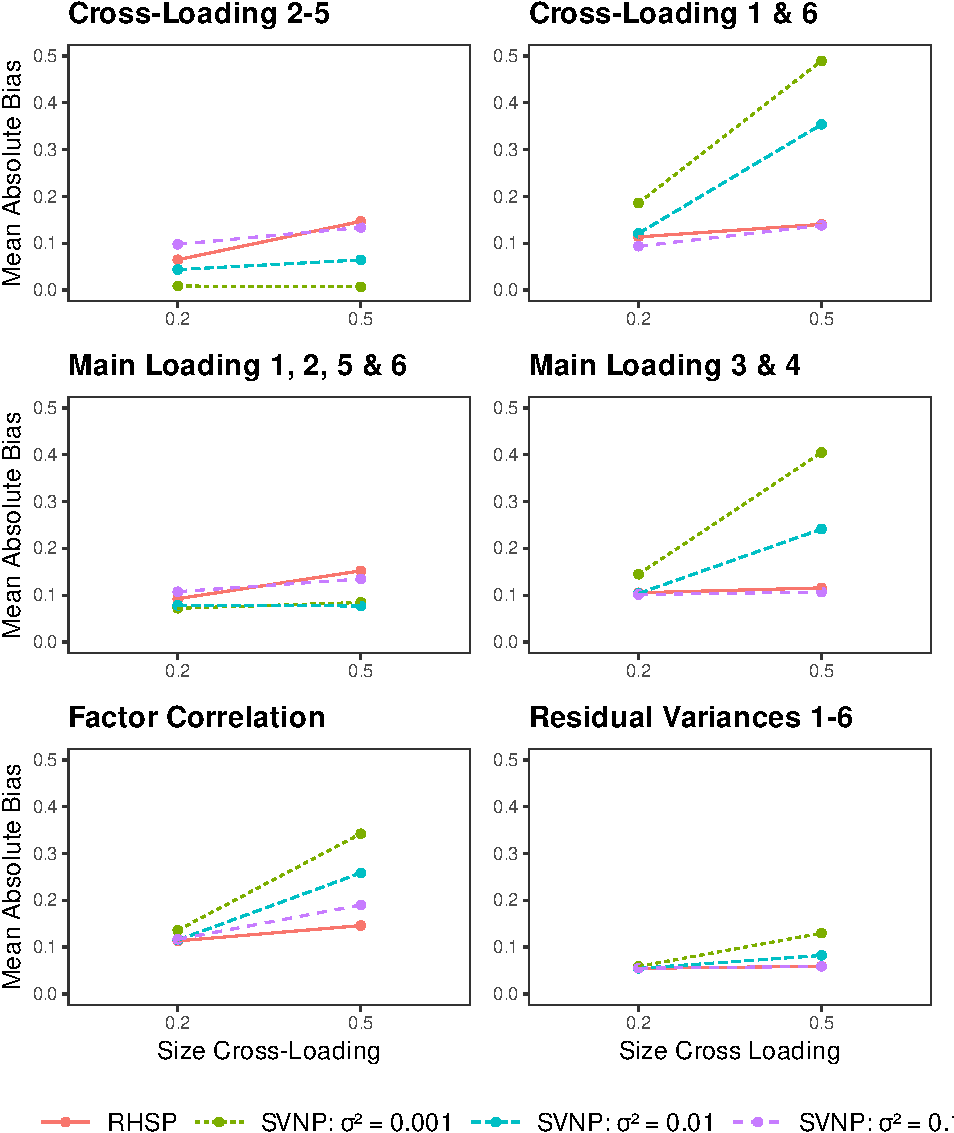
\includegraphics{Koch-vanErp_files/figure-latex/unnamed-chunk-5-1.pdf}
\caption{Mean Absolute Bias in the Model Parameters (N = 100). Per set
of parameters that showed an identical pattern, the first parameter was
used to represent all other parameters, e.g., cross-loading 2 was
plotted representative for cross-loading 3-5. All hyperparameters of the
RHSP are set to 1 in the results presented here.}
\end{figure}

The truly zero cross-loadings (\(\bar{\lambda}_{c 2-5}\)) had overall
little levels of bias, across priors and hyper-parameter settings. The
patterns in the bias of the RHSP was almost identical to that of the
SVNP with \(\sigma^2 = 0.1\). Note that for both priors the bias in
these cross-loadings comes from these cross-loading being
under-estimated (i.e., estimated as smaller than zero).

Regarding the truly non-zero cross-loadings (\(\bar{\lambda}_{c 1, 6}\))
the bias was sometimes very large for the SVNP, particularly with large
true cross-loadings of 0.5 and \(\sigma^2 = 0.001\) (e.g.,
\(\bar{Bias}_{\bar{\lambda}_{c 1}} = 0.49\)), since the estimates of the
true cross-loadings of 0.5 were shrunken almost entirely to zero (e.g.,
\(\bar{\lambda}_{c 1} = 0.01\)). Also with \(\sigma^2 = 0.01\) (and true
cross-loadings of 0.5) substantial bias occured (e.g.,
\(\bar{Bias}_{\bar{\lambda}_{c 1}} = 0.35\)), as the cross-loadings were
still under-estimated considerably (e.g.,
\(\bar{\lambda}_{c 1} = 0.15\)), though not entirely shrunken to zero.
With \(\sigma^2 = 0.1\) the bias in the estimates of the truly non-zero
cross-loadings of 0.5 was less pronounced (e.g.,
\(\bar{Bias}_{\bar{\lambda}_{c 1}} = 0.14\)). Here \(\sigma^2\) was
large enough to estimate the cross-loadings closer to their true value,
e.g., \(\bar{\lambda}_{c 1} = 0.37\). The bias of the RHSP was again
almost entirely identical to that of the SVNP with \(\sigma^2 = 0.1\).

Also the estimates of the main loadings of factor 1 on item 3
(\(\bar{\lambda}_{m 3}\)) and of factor 2 on item 4
(\(\bar{\lambda}_{m 4}\)) were substantially biased under the SVNP when
the true cross-loadings were 0.5 and \(\sigma^2 = 0.001\) (e.g.,
\(\bar{Bias}_{\bar{\lambda}_{m 3}} = 0.40\)). These two loadings showed
much higher bias than the other four main-loadings, as they loaded on
the same two items as the two non-zero cross-loadings
(\(\bar{\lambda}_{c 1}\) and \(\bar{\lambda}_{c 6}\), see Figure 2). As
the cross-loadings were shrunken to zero, these main loadings now also
accounted for the variance in the items that was truly explained by the
cross-loadings. Consequently, the two main-loadings were over-estimated,
e.g., \(\bar{\lambda}_{m 3} = 1.15\). Both the RHSP and the SVNP with
\(\sigma^2 = 0.1\) had low levels of bias for the main-loadings both
with true cross-loadings of 0.2 and 0.5.

In the factor correlation \(\bar{\Psi}_{1,2}\) the bias was relatively
small and approximately the same for the RHSP and the SVNP with
different values of \(\sigma^2\) when the truly non-zero cross-loadings
were 0.2. For the SVNP, bias became again much more pronounced with true
cross-loadings of 0.5 and small values of \(\sigma^2\), particularly
\(\sigma^2 = 0.001\) (\(\bar{Bias}_{\bar{\Psi}_{1,2}} = 0.34\)). In this
situation the factor correlation was heavily over-estimated
(\(\bar{\Psi}_{1,2} = 0.84\)). This can be explained by the fact that
the covariance between item 3 and 4 that arose from the two
cross-loadings, was misattributed to the factor-correlation, as the
cross-loadings were shrunken to zero. For both the SVNP with
\(\sigma^2 = 0.1\) and the RHSP, the bias in the factor correlation was
much lower, although there was still a noticeable increase between true
cross-loadings of 0.2 and 0.5.

For both priors, the bias in the estimates of the residual variances
\(\bar{\theta}_{1-6}\) was not large across different conditions,
although for the SVNP there was a noticeable increase between true
cross-loadings of 0.2 and 0.5 when \(\sigma^2 = 0.001\).

\hypertarget{power-and-type-i-error-rate-1}{%
\subsubsection{Power and Type-I-Error
Rate}\label{power-and-type-i-error-rate-1}}

\begin{figure}
\centering
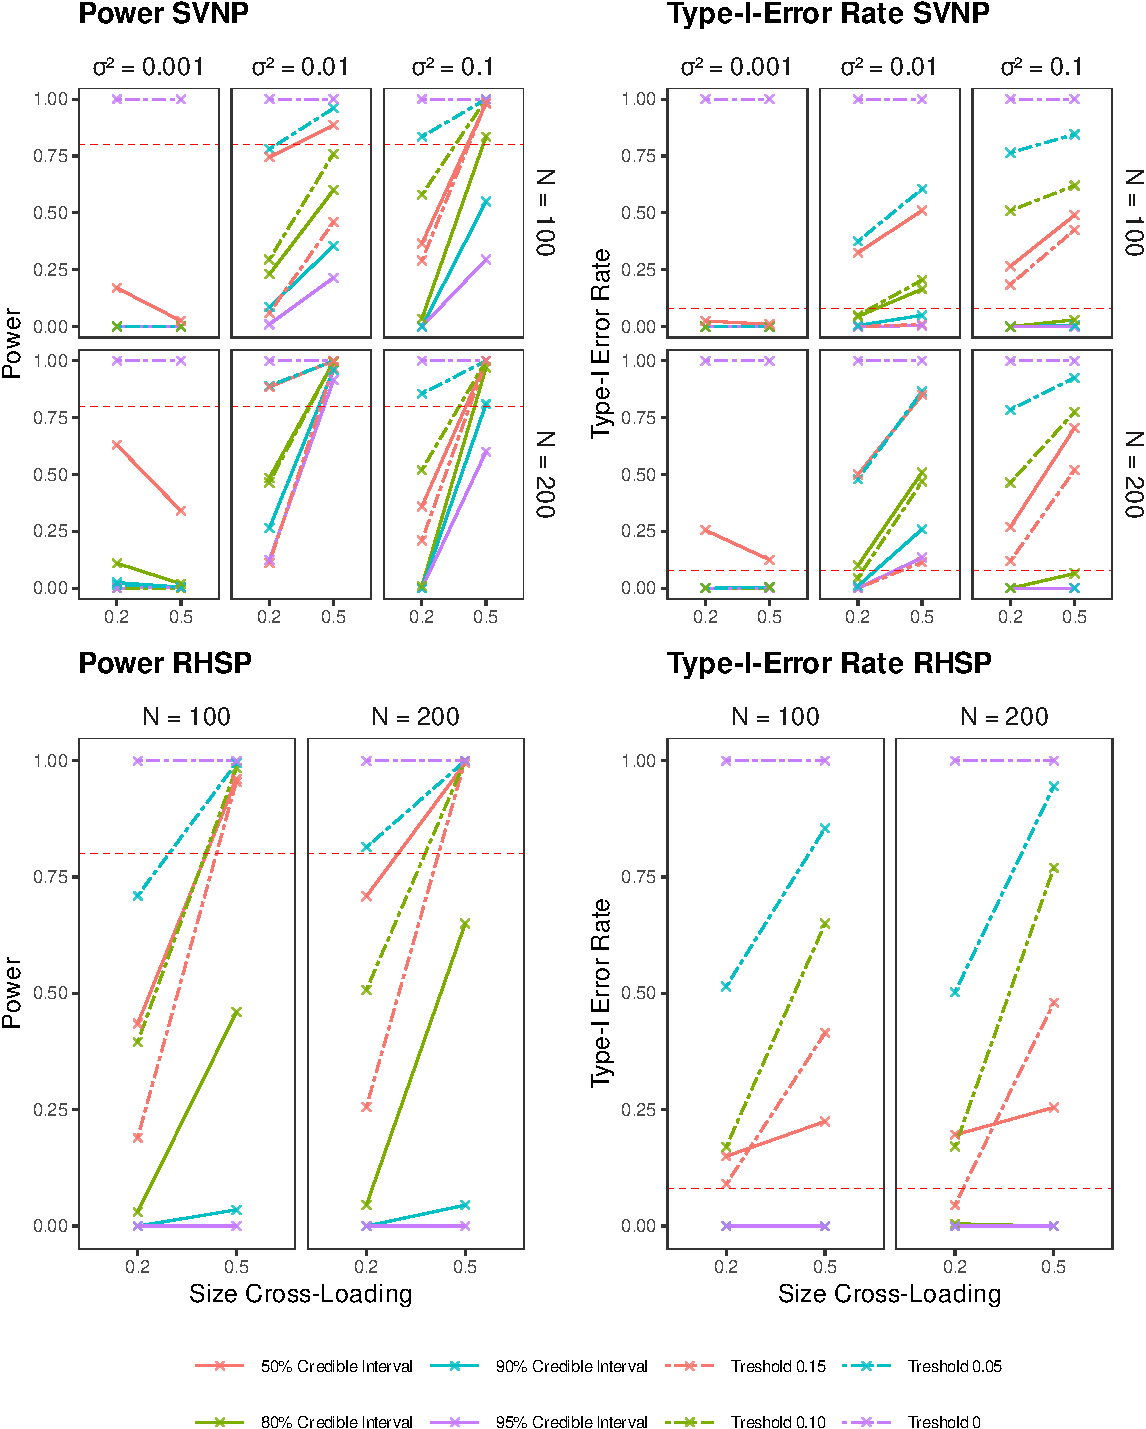
\includegraphics{Koch-vanErp_files/figure-latex/unnamed-chunk-6-1.pdf}
\caption{Mean Power and Type-I-Error Rates in Selecting non-zero
Crossloadings. All hyper-parameters of the RHSP are set to 1 in the
results presented here.}
\end{figure}

Figure 4 summarizes the Power and the Type-I-Error rate of both priors.
Again, the outcomes are presented for the first parameter of an
identical set of parameters (e.g., \(\lambda_{c,1}\) is presented
representative for the two truly non-zero cross-loadings). Moreover,
results of the RHSP are again presented with all hyper-parameters set to
one. In the plots summarizing the Power the horizontal red dashed line
indicates the minimum power of .80 recommended by
\citet{muthen_bayesian_2012}. According to \citet{cham_estimating_2012},
the maximally acceptable Type-I-Error rate is the upper-bound of a 95\%
interval of a binomial distribution, in this case
\(0.05 + 1.96 \times \sqrt{0.05 \times (1-0.05)/ N_{rep}} = 0.08\). This
maximum is visualized by the horizontal red dashed line in the
Type-I-Error rate plots. For both priors, with a threshold of 0.00 there
is both a Power and Type-I-Error rate of 1. This is logical, since
posterior means will never be entirely zero \citep{zhang_criteria_2021}.
The result thus mostly serves to illustrate this property of Bayesian
inference and thereby the need for more complex selection rules in
Bayesian regularization, if the goal is variable selection itself, and
not only unbiased model parameter estimates. Whether a high Power or a
low Type-I-Error rate is prioritized depends on many factors, such as
the model at hand and the research goal. In general, one should aim for
a balance between both, with high enough levels of Power and low enough
Type-I-Error rates co-occuring.

For both priors and across most conditions, the Power fell under the
desired threshold of .80. For the SVNP with \(\sigma^2 = 0.001\)
non-zero cross-loadings were always over-shrunken so much that they were
never selected as non-zero. Under \(\sigma^2 = 0.01\), the situation
improved somewhat, with now cross-loadings of 0.5 being correctly
selected as non-zero for all selection rules when N = 200. For N = 100,
thresholds of 0.05, and 50\% credible intervals also had the desired
levels of power, with thresholds of 0.10 also almost reaching a power of
.80. The SVNP performed best in terms of power when \(\sigma^2 = 0.1\).
With N = 200, all selection rules except for the 95\% credible intervals
reached the desired Power. With N = 100, all selection rules except for
the 95\% and 90\% credible intervals exceeded a power of .80. For the
RHSP, in general the Power did also not live up to the standards by
\citet{muthen_bayesian_2012}. The desired power was exclusively reached
in selecting cross-loadings that were truly 0.5, when using 50\%
credible intervals or the three thresholds. Especially the widest (90\%
and 95\%) credible intervals performed very poorly, which is explained
by the fact that the lower bounds of these intervals (almost) always
exceeded zero.

In general, under most conditions the Type-I-Error rate of both the SVNP
and the RHSP exceeded the desired maximum. For the SVNP, with
\(\sigma^2 = 0.001\) and N = 100, the Type-I-Error rate stayed very low
for all selection critera (up to the 0.00 threshold), as under this
condition all cross-loadings, including the truly zero ones, were always
shrunken almost entirely to zero. With N = 200, the 50\% credible
intervals lead to an undesired large Type-I error rate. With
\(\sigma^2 = 0.01\) and N = 100, some selection rules (90\% \& 95\%
credible intervals, a threshold of 0.15) had an acceptable Type-I-Error
rate even with large true cross-loadings of 0.5, but they quickly became
unacceptably high with N = 200. With \(\sigma^2 = 0.1\), all selection
rules except for 90\% and 95\% credible intervals had unacceptably high
Type-I-Error rates for both sizes of non-zero cross-loadings, even
though pronounced differences between cross-loadings of 0.2 and 0.5
occured. This was the condition under which the SVNP had the best levels
of power, indicating that the good performance in Power comes with the
caveat of a poor Type-I-Error rate. The RHSP performed even worse than
the SVNP in terms of its Type-I-Error rate. Only the 90\% and 95\%
credible intervals stayed within the desired boundary, as they always
included zero. This, however, is not useful in practice as these
intervals were completely unable to identify truly non-zero
cross-loadings correctly as non-zero.

\hypertarget{conclusions-and-discussion}{%
\section{Conclusions and Discussion}\label{conclusions-and-discussion}}

This was the first study to apply the Regularized Horseshoe Prior
\citep[RHSP,][]{piironen_sparsity_2017} in Bayesian Regularized SEM, by
using it to select cross-loadings in CFA. A comparison to the Bayesian
CFA approach by \citet{muthen_bayesian_2012} was made, where
cross-loadings are regularized with the Small Variance Normal Prior
(SVNP).

Both the SVNP and the RHSP performed well with small truly non-zero
cross-loadings of 0.2, in terms of estimating the model without
substantial bias. This can be interpreted as a successful instance of
regularization, where an acceptable amount of bias is added to the model
by shrinking some parameters to(wards) zero, to reach a sparser
solution. However, under some hyper-parameter settings the performance
of the SVNP decreased substantially with larger truly non-zero
cross-loadings of 0.5. With smaller values of \(\sigma^2\), particularly
with \(\sigma^2 = 0.001\), these cross-loadings were still shrunken to
zero, even though they were much larger in reality. This caused
substantial bias, not only in the estimates of the cross-loadings
itself, but also in the estimates of some main-loadings and the factor
correlation. In practice, bias in structural parameters is particularly
concerning, as it may lead to wrong conclusions in research on
structural relationships between latent constructs. With
\(\sigma^2 = 0.1\), the SVNP was able to estimate the model parameters
with little bias. Such relatively large variance still allowed for
enough deviations from zero in the cross-loadings to yield relatively
accurate estimates of the non-zero cross-loadings itself and,
consequently, the other model parameters. The RHSP performed very
similar to the SVNP with \(\sigma^2 = 0.1\).

While the RHSP and the SVNP were both able to estimate the simple CFA
model of this study with little bias, only the RHSP was able to do so
consistently across different hyper-parameter settings. This poses a
central advantage over the SVNP. Being robust to different
hyper-parameter settings, which is achieved though the complex nature of
the RHSP that sets hyper-priors on all parameters, may ultimately allow
researchers to apply the RHSP without having to worry about choosing
optimal values for the hyper-parameters. However, the other side of the
coin is that the complex nature of the RHSP makes it sensitive to
hyper-parameter settings regarding its performance in terms of
convergence, in contrast to the SVNP that had excellent convergence
across all conditions. Hereby, a clear pattern arose, with convergence
issues arising with large cross-loadings, small sample sizes and small
scales for the local and global shrinkage parameter. While this may
suggest that one should simply avoid using small values for the scales,
using larger scales that shrink parameters less may lead to
identification problems in more complex SEM models. Future research is
required that incorporates more complex models, in order to assess the
performance of the RHSP in terms of convergence in more depth.
Ultimately, it is desirable to be able to formulate clear guidelines on
which hyper-parameter configurations to use in which situations to avoid
convergence issues, to make the RHSP a practical approach.

Particularly under simple models such as the one employed in this study
using the less complex SVNP with a relatively large value of
\(\sigma^2\) may thus prove advantageous in practice, to avoid risking
bias stemming from non-convergence and divergent transitions. Next to
this, the simpler SVNP is easier to implement and takes substantially
less time to run. However, simply using larger values of \(\sigma^2\)
with the SVNP is no general solution. In practice, models may include
more structural parameters, even more cross-loadings, or a number of
residual co-variances. Under these circumstances, large values of
\(\sigma^2\) may lead to identification issues. Moreover, the larger
\(\sigma^2\), the more cross-loadings will be selected as non-zero,
which may ultimately lead to over-fitting. Because of this, the RHSP
might prove as more advisable for more complex models. While the RHSP,
as the SVNP, can be assumed to run into more and more identification
issues with increasing model complexity, its refined nature in giving
prior mass only where strictly desired (see Figure 1) might allow for a
more efficient identification of complex models than the SVNP, at least
for some hyper-parameter settings. Using the RHSP may thus turn out to
be the approach of choice in situations where identification is hard to
achieve with the SVNP. However, future research comparing the SVNP to
the RHSP in regularizing more complex SEM-models is yet to investigate
this directly.

Regarding the Power and Type-I-Error rate in selecting cross-loadings as
non-zero, both priors performed poorly across a range of selection
rules. First of all, this is not surprising, given earlier research
which clearly showed that a range of shrinkage priors \citep[SVNP,
Bayesian LASSO, Spike-and-Slab
Prior,][]{lu_bayesian_2016, zhang_criteria_2021} generally need much
larger sample sizes than the ones employed in this study to reach
desirable levels of Power and Type-I-Error rates \citep[see][who show
that frequentist variable selection methods are sensitive to sample size
too]{jacobucci_regularized_2016, lu_bayesian_2016}. Future research
should therefore assess the Power and Type-I-Error rate of the RHSP
under larger sample sizes (e.g., N = 500, 1000, 2000) to allow for a
more conclusive picture. At the same time, it is an important finding
that both priors perform poorly under small sample sizes, as simple CFA
models are often fitted with such small sample sizes in practice. Note
also that our findings do not imply that the RHSP is useless under small
sample sizes. If the goal of regularization is not to select which
cross-loadings are non-zero, but to yield unbiased estimates of the
other model parameters, the RHSP still works better than the SVNP under
most settings, even with small sample sizes. In practice, researchers
often fit SEM-models including a measurement structure to test
structural hypotheses. For this purpose, the question of whether or not
cross-loadings are zero is not as relevant, as long as the structural
model parameters are estimated without substantial bias. Next to this,
different selection methods, such as Highest Posterior Density (HPD)
intervals \citep{zhang_criteria_2021}, or projection predictive
inference \citep{piironen_sparsity_2017} may be more successful in
making a selection that meets the desired balance in Power and
Type-I-Error rate.

The large levels of bias found in the SVNP (for the majority of
hyper-parameter settings) are not surprising, given the original
approach explicitly asking for a second step to circumvent bias
\citep{muthen_bayesian_2012}. However, the fact that the SVNP performed
so poorly in selecting the cross-loadings across selection rules
suggests that in practice the 2-step approach, which heavily relies on a
correct selection of cross-loadings as non-zero, is not advisable. This,
however, needs to be directly assessed in future research. One approach
of doing so would be to first make a selection of cross-loadings and
then actively execute the second estimation step using new validation
data sets. This would allow to compare the bias of the 2-step SVNP to
the (1-step) RHSP directly. While our study formed a valuable first step
in establishing the performance of the RHSP in regularized SEM, such a
design would allow to more directly answer the question of whether or
not the RHSP enables us to `get a step ahead'.

Next to specific limitations named above, the current study has some
general shortcomings, which lead to a number of recommendations for
future research. First, we only assessed the performance of the RHSP in
regularizing cross-loadings in a very simple CFA model consisting of
only two factors. A straightforward way of extending the current study
and making its findings more generalizable would be to include factor
models with more factors. Within CFA models, another important set of
parameters that can be identified through the usage of shrinkage priors
are residual co-variances (i.e., the off-diagonal elements of
\(\Theta\)), which are usually fixed to zero in classic CFA
\citep{muthen_bayesian_2012}. An important next step is thus to assess
the performance of the RHSP in selecting residual co-variances on top of
cross-loadings. Hereby, it is advisable to start by regularizing
residual co-variances separately rather than on top of cross-loadings,
as regularizing both parameters simultaneously can be challenging in
practice \citep{zhang_criteria_2021}. It is also desirable to assess the
performance of the RHSP in regularizing model parameters in more complex
SEM models, such as structural parameters, e.g., indirect effects in
mediation models, or regression coefficients in MIMIC models. Also
applying the RHSP in measurement models with non-continuous (i.e.,
binary, ordinal or nominal) outcomes would be an interesting way of
building on the current study. Regarding the SVNP, incorporating
extensions of the SVNP where a hyper-prior is set for \(\sigma^2\)
\citep[see for instance][]{lu_bayesian_2016} may prove valuable in
allowing for a more refined comparison between the SVNP and the RHSP.
Note also that in the current study no direct comparison to other
relevant shrinkage priors, such as the Bayesian LASSO or the
Spike-And-Slab Prior was made. Further down the line the RSHP should be
implemented into standard Bayesian SEM software \citep[e.g., by adding
it to the BLAVAAN package,][]{merkle_efficient_2020}, such that applied
researchers can actually take advantage of it in practice.

Despite the limitations named, the current study forms a valuable
contribution to the current literature. We set a crucial first step in
establishing the usefulness of the RHSP in Bayesian regularized SEM. Our
findings show that the RHSP can generally be successfully be applied in
Bayesian regularized SEM and point to important directions for future
research.

\bibliographystyle{tfcad}
\bibliography{refs.bib}





\end{document}
